% document style header
\documentclass[a4paper, 12pt]{config/homework}

% import default packages
\usepackage{config/defpackages}

% import custom math commands
\usepackage{config/domath}

% end preamble
\begin{document}

% document title
\noindent
\begin{tabularx}{\textwidth}{>{\centering\arraybackslash}X>{\centering\arraybackslash}X>{\centering\arraybackslash}X}
Calvin Sprouse & PHYS474 Homework 1 & Due 2024 Jan 10\\
\midrule
\end{tabularx}

% homework problems begin
Note that integrals have been evaluated by the provided integral table.
\begin{enumerate}
\item Consider the continuous Gaussian distribution, \(\rho(x) = Ae^{-\lambda (x-a)^2}\), where \(A\), \(a\), and \(\lambda \) are positive, real constants. Note that this is \underline{not} a wavefunction, but rather a distribution.
\begin{enumerate}[label=(\alph*)]
\item Normalize the distribution to determine \(A\).
\begin{align*}
1 &= \bint{-\infty}{\infty}{\rho(x)}{x}
\\&= \bint{-\infty}{\infty}{Ae^{-\lambda (x-a)^2}}{x}
\\&= A \bint{-\infty}{\infty}{e^{-\lambda (x-a)^2}}{x}
\\&= A \bint{-\infty}{\infty}{e^{-(\lambda x^2 -2\lambda ax + \lambda a^2)}}{x}
\\&= A \sqrt{\frac{\pi}{\lambda}} \exp\left({\frac{(-2\lambda a)^2 - 4\lambda^2 a^2}{4\lambda}}\right)
\\&= A \sqrt{\frac{\pi}{\lambda}}.
\end{align*}
Thus, \(A = \sqrt{\lambda / \pi}\).

\item Determine \(\braket{x}\), \(\braket{x^2}\), and \(\sigma \).

The average value of \(x\), or expectation value, is given by
\begin{align*}
\braket{x} &= \bint{-\infty}{\infty}{x \rho(x)}{x}
\\&= \sqrt{\frac{\lambda}{\pi}} \bint{-\infty}{\infty}{x \exp{\left(-\lambda(x-a)^2\right)}}{x}
\\&= \sqrt{\frac{\lambda}{\pi}} a \sqrt{\frac{\pi}{\lambda}}
\\&= a.
\end{align*}

The average of the squares of \(x\) is given by
\begin{align*}
\braket{x^2} &= \bint{-\infty}{\infty}{x^2 \rho(x)}{x}
\\&= \sqrt{\frac{\lambda}{\pi}} \bint{-\infty}{\infty}{x^2 \exp{\left(-\lambda(x-a)^2\right)}}{x}
\\&= \sqrt{\frac{\lambda}{\pi}} \bint{-\infty}{\infty}{x^2 \exp{\left(-\lambda x^2 +2\lambda ax - \lambda a^2\right)}}{x}
\\&= \sqrt{\frac{\lambda}{\pi}} \bint{-\infty}{\infty}{x^2 \exp{\left(-\lambda x^2 + 2\lambda a x\right)}\exp{\left(-\lambda a^2\right)}}{x}
\\&= \sqrt{\frac{\lambda}{\pi}} \exp{\left(-\lambda a^2\right)} \bint{-\infty}{\infty}{x^2 \exp{\left(-\lambda x^2 + 2\lambda a x\right)}}{x}
\\&= \sqrt{\frac{\lambda}{\pi}} \exp{\left(-\lambda a^2\right)} \frac{\sqrt{\pi} (2\lambda + (2\lambda a)^2)}{4 \lambda^{5/2}} \exp{\left(\frac{(2\lambda a)^2}{4\lambda}\right)}
\\&= \frac{2\lambda + (2\lambda a)^2}{4\lambda^2}
\\&= \frac{1 + 2\lambda a^2}{2\lambda}.
\end{align*}

The standard deviation, \(\sigma \), of \(\rho \) is given by
\begin{align*}
\sigma &= \sqrt{\braket{x^2} - \braket{x}^2}
\\&= \sqrt{\frac{1 + 2\lambda a^2}{2\lambda} - a^2}
\\&= \frac{1}{\sqrt{2\lambda}}.
\end{align*}
\end{enumerate}

\pagebreak
\item At time \(t=\qty{0}{\second}\), an electron is represented by the wave function,
\[\Psi(x, 0) = \begin{cases}
    A\frac{x}{a}, & 0 \le x \le a \\
    A \frac{(b-x)}{(b-a)}, & a \le x \le b \\
    0, & \text{otherwise}
\end{cases}\]
where \(A\), \(a\), and \(b\) are constants.
\begin{enumerate}[label=(\alph*)]
\item Normalize \(\Psi \).
\begin{align*}
1 &= \bint{-\infty}{\infty}{\left| \Psi \right|^2}{x}
\\&= \bint{-\infty}{0}{(0)^2}{x} + \bint{0}{a}{\left(A \frac{x}{a}\right)^2}{x} + \bint{a}{b}{\left(A\frac{(b-x)}{(b-a)}\right)^2}{x} + \bint{b}{\infty}{(0)^2}{x}
\\&= 0 + \frac{A^2}{a^2}\bint{0}{a}{x^2}{x} + \frac{A^2}{(b-a)^2}\bint{a}{b}{(b-x)^2}{x} + 0
\\&= \frac{A^2}{a^2} \left[\frac{1}{3}x^3\right]_0^a + \frac{A^2}{(b-a)^2}\left[-\frac{a^3}{3} + a^2b - ab^2 + \frac{b^3}{3}\right]_a^b
\\&= \frac{A^2}{a^2} \frac{a^3}{3} + \frac{A^2}{(b-a)^2}\frac{(b-a)^3}{3}
\\&= A^2 \left(\frac{a}{3} + \frac{b-a}{3}\right)
\\&= A^2 \frac{b}{3}.
\end{align*}
Thus, \(A = \sqrt{3/b}\).

\item Sketch \(\Psi(x,0)\) as a function of \(x\).
\begin{figure}[h]
    \centering
    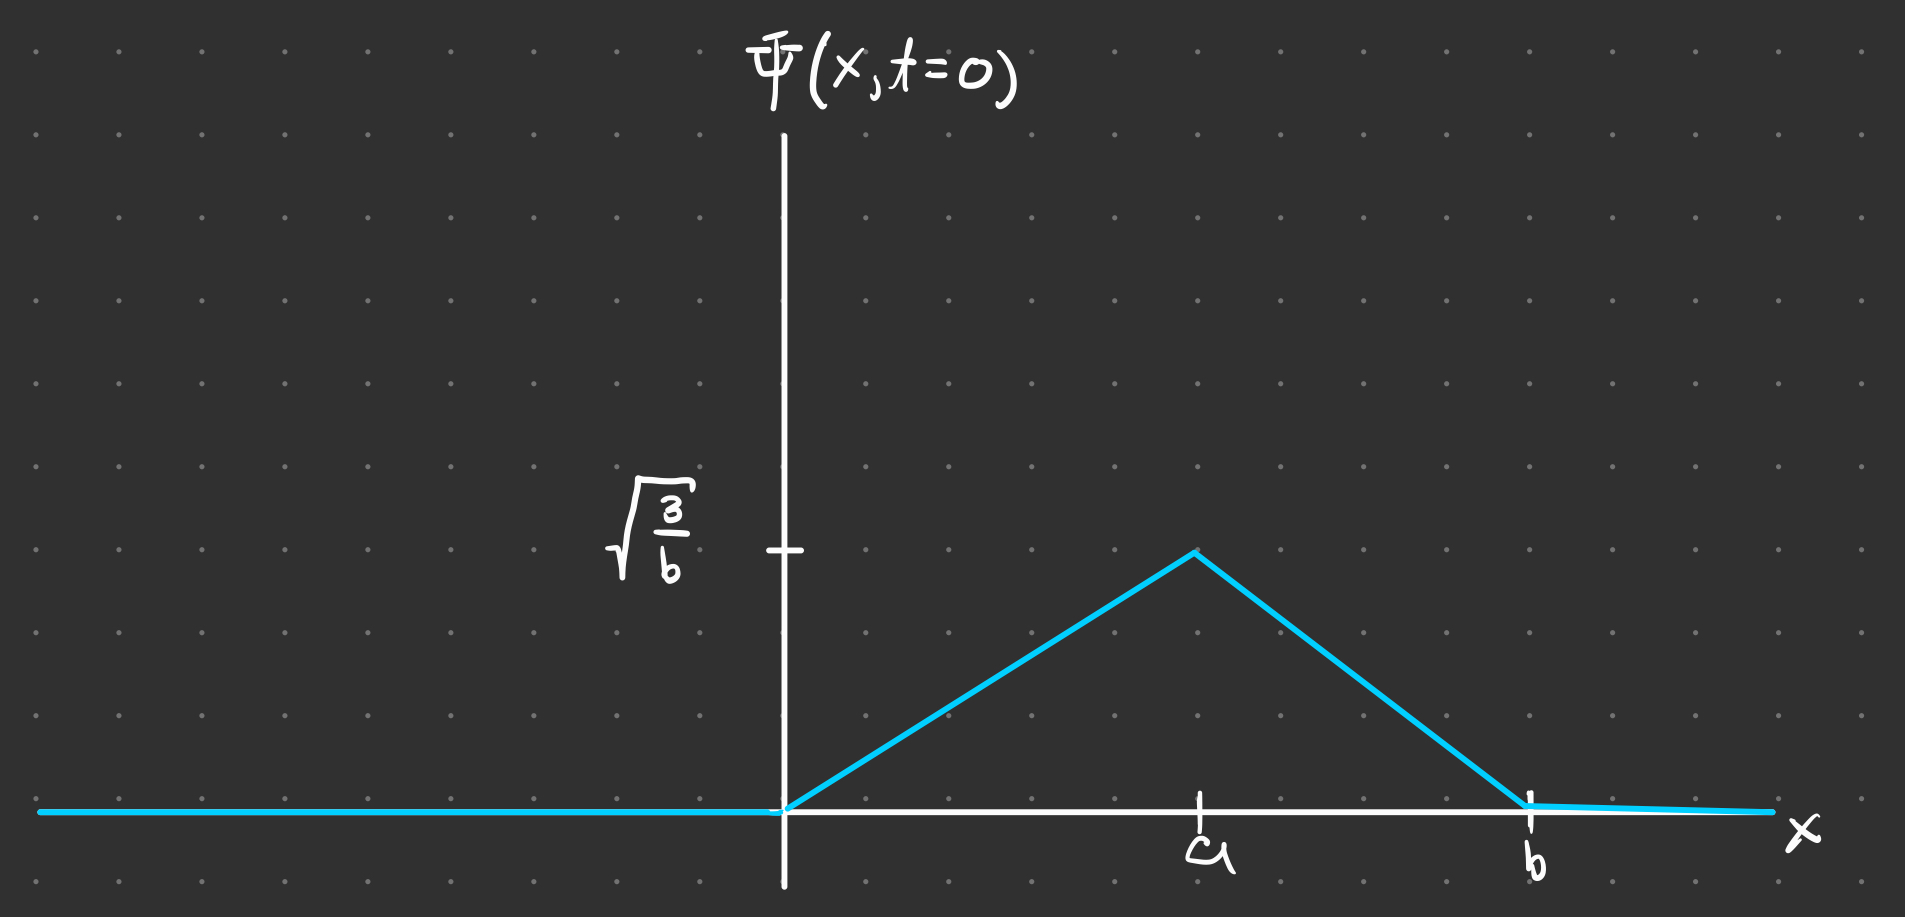
\includegraphics[width=0.8\textwidth]{qm_hw1_p2b.jpeg}
\end{figure}
\\Note, \(\Psi=0\) when \(x\ge b\) contrary to the sketch.

\pagebreak
\item Where is the electron most likely to be found at \(t=\qty{0}{\second}\)?
\\The most likely position of the electron is given by solving
\[\odv{\left|\Psi\right|^2}{x} = 0\]
for maximum values. We begin on the interval \(0 \le x \le a\).
\begin{align*}
\odv{\left(A \frac{x}{a}\right)^2}{x} &= 0,
\\\frac{3}{ba^2}\odv{x^2}{x} &= 0,
\\\frac{6}{ba^2} x &= 0,
\\x &= 0.
\end{align*}
The probability of finding the electron at \(x=0\) is given by
\begin{align*}
\left| \Psi(x=0,t=0) \right|^2 &= \frac{3}{ba^2} (0)^2
\\&= 0.
\end{align*}
We now check the interval \(a \le x \le b\).
\begin{align*}
\odv{\left(A \frac{b-x}{b-a}\right)^2}{x} &= 0,
\\\frac{3}{ba^2(b-a)^2}\odv{(b-x)^2}{x} &= 0,
\\\frac{-6}{ba^2(b-a)^2}(b-x) &= 0,
\\b-x &= 0,
\\x &= b.
\end{align*}
The probability of finding the electron at \(x=b\) is given by
\begin{align*}
\left| \Psi(x=b,t=0) \right|^2 &= \frac{3}{ba^2(b-a)^2}(b-b)^2
\\&= 0.
\end{align*}
We now check the probability of finding the electron at the  boundaries, that is, \(x=a\).
\begin{align*}
\left| \Psi(x=a, t=0) \right|^2 &= \frac{3}{ba^2}a^2
\\&= \frac{3}{b}.
\end{align*}
Thus, the electron is most likely to be found at \(x=a\). In hindsight, this could have been simpler since a valid wave-function is continuous. At the boundaries \(x=0\) and \(x=b\) we could have simply observed the ``otherwise'' case and seen that, to be continuous, \(\Psi(x=0,t=0)\) and \(\Psi(x=b,t=0)\) must be equal to 0. Thus, we would not have needed to calculate the probability of finding the electron at \(x=0\) or \(x=b\).

\item What is the probability the electron will be found in the region \(x \le a\)? Check your result in the limiting case where \(b=a\) and \(b=2a\).
\\The probability that the electron will be found in the region \(x \le a\) is given by
\begin{align*}
\bint{-\infty}{a}{\left|Psi\right|^2}{x} &= \bint{0}{a}{\left(\frac{Ax}{a}\right)^2}{x}
\\&= \frac{3}{ba^2}\bint{0}{a}{x^2}{x}
\\&= \frac{3}{ba^2}\left[\frac{1}{3}x^3\right]_0^a
\\&= \frac{3}{ba^2} \frac{a^3}{3}
\\&= \frac{a}{b}.
\end{align*}
If \(b=a\) the wave-function takes on non-zero values only in the interval \\ \(0 \le x \le a\) meaning the electron can only be found on the interval \(0 \le x \le a\). Thus the probability of finding the electron on the interval \(0 \le x \le a\) should be 1:
\[\frac{a}{b} = \frac{a}{a} = 1.\]
If \(b=2a\) the probability of finding the electron on the interval \(0 \le x \le a\) should be less than 1:
\[\frac{a}{b} = \frac{a}{2a} = \frac{1}{2}.\]

\item Determine \(\braket{x}\).
\begin{align*}
\braket{x} &= \bint{-\infty}{\infty}{x\left| \Psi \right|^2}{x}
\\&= \bint{0}{a}{x\left(\sqrt{\frac{3}{b}} \frac{x}{a}\right)^2}{x} + \bint{a}{b}{x\left(\sqrt{\frac{3}{b}}\frac{(b-x)}{(b-a)}\right)^2}{x}
\\&= \frac{3}{ba^2}\bint{0}{a}{x^3}{x} + \frac{3}{b}\frac{1}{(b-a)^2}\bint{a}{b}{(b^2 x - 2bx^2 + x^3)}{x}
\\&= \frac{3}{ba^2}\left[\frac{1}{4}x^4\right]_0^a + \frac{3}{b}\frac{1}{(b-a)^2} \left[\frac{b^2}{2}x^2 - \frac{2b}{3}x^3 + \frac{1}{4}x^4\right]_a^b
\\&= \frac{3}{4}\frac{a^2}{b} + 3 \frac{1}{b(b-a)^2}\left(\frac{b^4}{2} - \frac{2b^4}{3} + \frac{b^4}{4} - \frac{a^2 b^2}{2} + \frac{2ba^3}{3} - \frac{a^4}{4}\right)
\\&= \frac{3}{4} \frac{a^2}{b} + 3 \frac{1}{b(b-a)^2}\frac{(b-a)^3(3a+b)}{12}
\\&= \frac{3}{4} \frac{a^2}{b} + \frac{1}{4} \frac{(b-a)(3a+b)}{b}
\\&= \frac{3a^2 + (b-a)(3a+b)}{4b}
\\&= \frac{1}{4} (2a+b).
\end{align*}

\end{enumerate}
\end{enumerate}
\end{document}
